% Latex header for doxygen 1.8.9.1
\documentclass[twoside]{book}

% Packages required by doxygen
\usepackage{fixltx2e}
\usepackage{calc}
\usepackage{doxygen}
\usepackage[export]{adjustbox} % also loads graphicx
\usepackage{graphicx}
\usepackage[utf8]{inputenc}
\usepackage{makeidx}
\usepackage{multicol}
\usepackage{multirow}
\PassOptionsToPackage{warn}{textcomp}
\usepackage{textcomp}
\usepackage[nointegrals]{wasysym}
\usepackage[table]{xcolor}

% Font selection
\usepackage[T1]{fontenc}
\usepackage[scaled=.90]{helvet}
\usepackage{courier}
\usepackage{amssymb}
\usepackage{sectsty}
\renewcommand{\familydefault}{\sfdefault}
\allsectionsfont{%
  \fontseries{bc}\selectfont%
  \color{darkgray}%
}
\renewcommand{\DoxyLabelFont}{%
  \fontseries{bc}\selectfont%
  \color{darkgray}%
}
\newcommand{\+}{\discretionary{\mbox{\scriptsize$\hookleftarrow$}}{}{}}

% Page & text layout
\usepackage{geometry}
\geometry{%
  a4paper,%
  top=2.5cm,%
  bottom=2.5cm,%
  left=2.5cm,%
  right=2.5cm%
}
\usepackage[T1]{fontenc}
\usepackage{titlesec, blindtext, color}
\definecolor{gray75}{gray}{0.75}
\newcommand{\hsp}{\hspace{20pt}}
\titleformat{\chapter}[hang]{\Huge\bfseries}{\thechapter\hsp\textcolor{gray75}{|}\hsp}{0pt}{\Huge\bfseries}
\tolerance=750
\hfuzz=15pt
\hbadness=750
\setlength{\emergencystretch}{15pt}
\setlength{\parindent}{0cm}
\setlength{\parskip}{0.2cm}
\makeatletter
\renewcommand{\paragraph}{%
  \@startsection{paragraph}{4}{0ex}{-1.0ex}{1.0ex}{%
    \normalfont\normalsize\bfseries\SS@parafont%
  }%
}
\renewcommand{\subparagraph}{%
  \@startsection{subparagraph}{5}{0ex}{-1.0ex}{1.0ex}{%
    \normalfont\normalsize\bfseries\SS@subparafont%
  }%
}
\makeatother

% Headers & footers
\usepackage{fancyhdr}
\pagestyle{fancyplain}
\fancyhead[LE]{\fancyplain{}{\bfseries\thepage}}
\fancyhead[CE]{\fancyplain{}{}}
\fancyhead[RE]{\fancyplain{}{\bfseries\leftmark}}
\fancyhead[LO]{\fancyplain{}{\bfseries\rightmark}}
\fancyhead[CO]{\fancyplain{}{}}
\fancyhead[RO]{\fancyplain{}{\bfseries\thepage}}
\fancyfoot[LE]{\fancyplain{}{}}
\fancyfoot[CE]{\fancyplain{}{}}
\fancyfoot[RE]{\fancyplain{}{\bfseries\scriptsize Generated by Yu Chen }}
\fancyfoot[LO]{\fancyplain{}{\bfseries\scriptsize Generated by Yu Chen }}
\fancyfoot[CO]{\fancyplain{}{}}
\fancyfoot[RO]{\fancyplain{}{}}
\renewcommand{\footrulewidth}{0.4pt}
\renewcommand{\chaptermark}[1]{%
  \markboth{#1}{}%
}
\renewcommand{\sectionmark}[1]{%
  \markright{\thesection\ #1}%
}

% Indices & bibliography
\usepackage{natbib}
\usepackage[titles]{tocloft}
\setcounter{tocdepth}{3}
\setcounter{secnumdepth}{5}
\makeindex

% Hyperlinks (required, but should be loaded last)
\usepackage{ifpdf}
\ifpdf
  \usepackage[pdftex,pagebackref=true]{hyperref}
\else
  \usepackage[ps2pdf,pagebackref=true]{hyperref}
\fi
\hypersetup{%
  colorlinks=true,%
  linkcolor=blue,%
  citecolor=blue,%
  unicode%
}

% Custom commands
\newcommand{\clearemptydoublepage}{%
  \newpage{\pagestyle{empty}\cleardoublepage}%
}


%===== C O N T E N T S =====

\usepackage[yyyymmdd,hhmmss]{datetime}

\begin{document}

% Titlepage & ToC
\hypersetup{pageanchor=false,
             bookmarks=true,
             bookmarksnumbered=true,
             pdfencoding=unicode
            }
\pagenumbering{roman}
\begin{titlepage}
\vspace*{7cm}
\begin{center}%
{\Huge Dual State Framework}\\
\vspace*{0.5cm}
{\Large Project Report}\\
\vspace*{1cm}
{\normalsize Yu Chen - C00151352}\\
\vspace*{0.2cm}
{\small \today\ \currenttime}\\
\end{center}
\end{titlepage}
\clearemptydoublepage
\chapter*{Abstract}
\label{_abstract}
\hypertarget{_abstract}{}
This report was commissioned to investigate the possibility of developing the library Dual State Framework that helps programmers implement parallel computing easily. The research covers\+:
\begin{DoxyItemize}
\item programming languages
\item libraries for Graphics
\item libraries of parallel programming
\item integrated development environments
\item source control tools
\item documentation tools
\item software packaging tools
\end{DoxyItemize}

According to the investigation, I think it is not hard to complete the project. The correct combination of Open Source and free applications seems to be the best choice to develop the framework.
\begin{DoxyItemize}
\item C++
\item S\+F\+M\+L
\item Intel T\+B\+B
\item Xcode
\item Git
\item Doxygen, Graphviz, and La\+Tex
\item Package\+Maker, Installforge, Debreate 
\end{DoxyItemize}
\tableofcontents
\clearemptydoublepage
\pagenumbering{arabic}
\hypersetup{pageanchor=true}

%--- Begin generated contents ---
\chapter{Introduction}
\label{_introduction}
\hypertarget{_introduction}{}
The document describes all functionalities estimated to be implemented for the project. It also shows what level of quality of the project should be achieved. Project plan and schedule are embedded in this document. \hypertarget{_introduction_IntroductionPurpose}{}\section{Purpose}\label{_introduction_IntroductionPurpose}
The main purpose of my project is to create a C++ framework for parallel computing. Parallel computing is the science and art of programming computers that can do more than one operation at once during the same cycle, simultaneously and concurrently. It performs often via having more than one processor. ~\newline
~\newline
Next, A benchmark program is required for profiling this framework. The program will be designed as a G\+U\+I application which shows the performance in different situations \hypertarget{_introduction_IntroductionPlan}{}\section{Plan}\label{_introduction_IntroductionPlan}
Dual State Framework will be developed by C++ under Mac Os X. Open\+M\+P or Intel T\+B\+B is used for implementing Parallel Computing. In addition, it will be compiled and debugged both on Microsoft Windows and Linux as well. This process will be done by Cmake. The A\+P\+I Documentation of this project will be created by Doxygen. ~\newline
~\newline
The simple benchmark program will be written by C++ with S\+F\+M\+L or S\+D\+L library. Git will be used for source control and version control. The project is now available in following link. ~\newline
~\newline
\href{https://github.com/kuyoonjo/DualStateFramework}{\tt https\+://github.\+com/kuyoonjo/\+Dual\+State\+Framework} \hypertarget{_introduction_IntroductionPotentialUsers}{}\section{Potential Users}\label{_introduction_IntroductionPotentialUsers}
Dual State Framework can have a variety of uses. Initially the project is concerned around computer games, but it can be used in broad kinds of software. The framework can be used in any program or game that runs parallel processes. Currently almost all of them meet that criteria. 
\chapter{Project Description}
\label{_project_description}
\hypertarget{_project_description}{}
\hypertarget{_project_description_ProjectDescriptionInstallations}{}\section{Installations}\label{_project_description_ProjectDescriptionInstallations}
The installers were uploaded on Source\+Forge \cite{sourceforge}. The download page is available at\+: \href{https://sourceforge.net/projects/dualstateframework/}{\tt https\+://sourceforge.\+net/projects/dualstateframework/}. Click the \char`\"{}files\char`\"{} tab, you will see all versions for different platform. 
\begin{DoxyImageNoCaption}
  \mbox{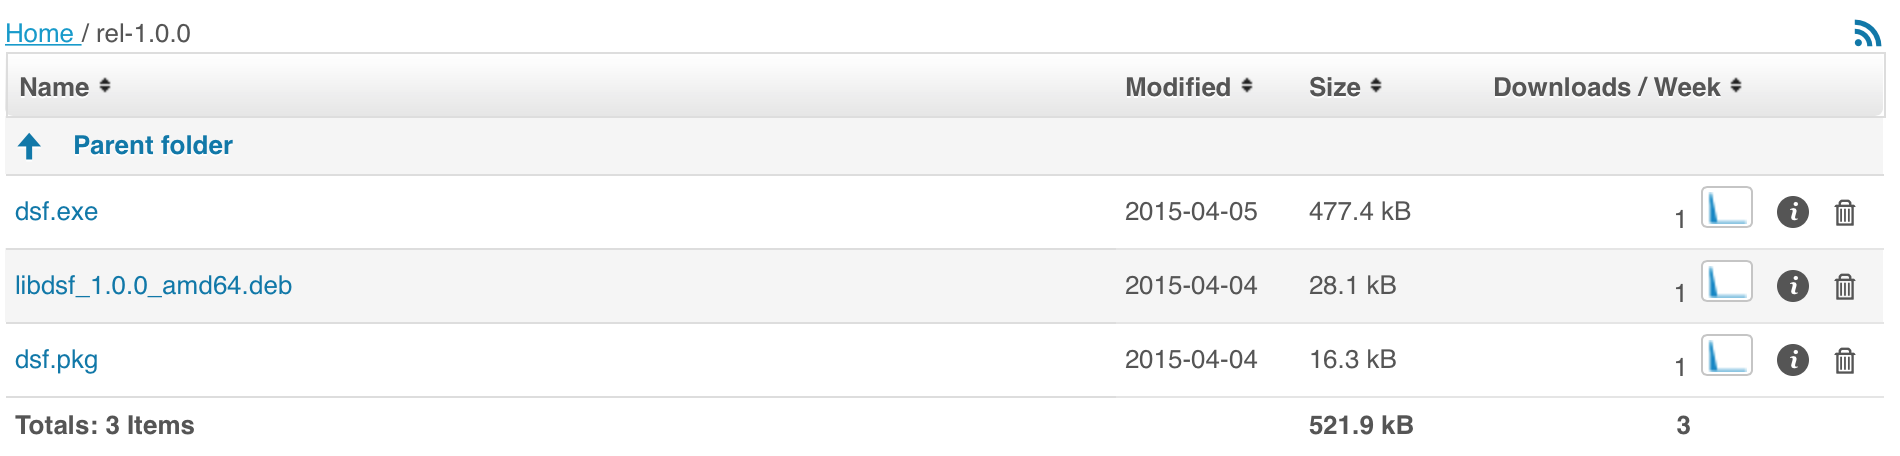
\includegraphics[width=\textwidth,height=\textheight/2,keepaspectratio=true]{ReportDescriptionInstallations.png}}
\end{DoxyImageNoCaption}
\hypertarget{_project_description_ProjectDescriptionFrameworkwithXcode}{}\section{Framework with Xcode}\label{_project_description_ProjectDescriptionFrameworkwithXcode}
The library is designed as a bundle \cite{bundle} for Mac O\+S X. To use it in Xcode you just need to drag it into your project explorer. 
\begin{DoxyImageNoCaption}
  \mbox{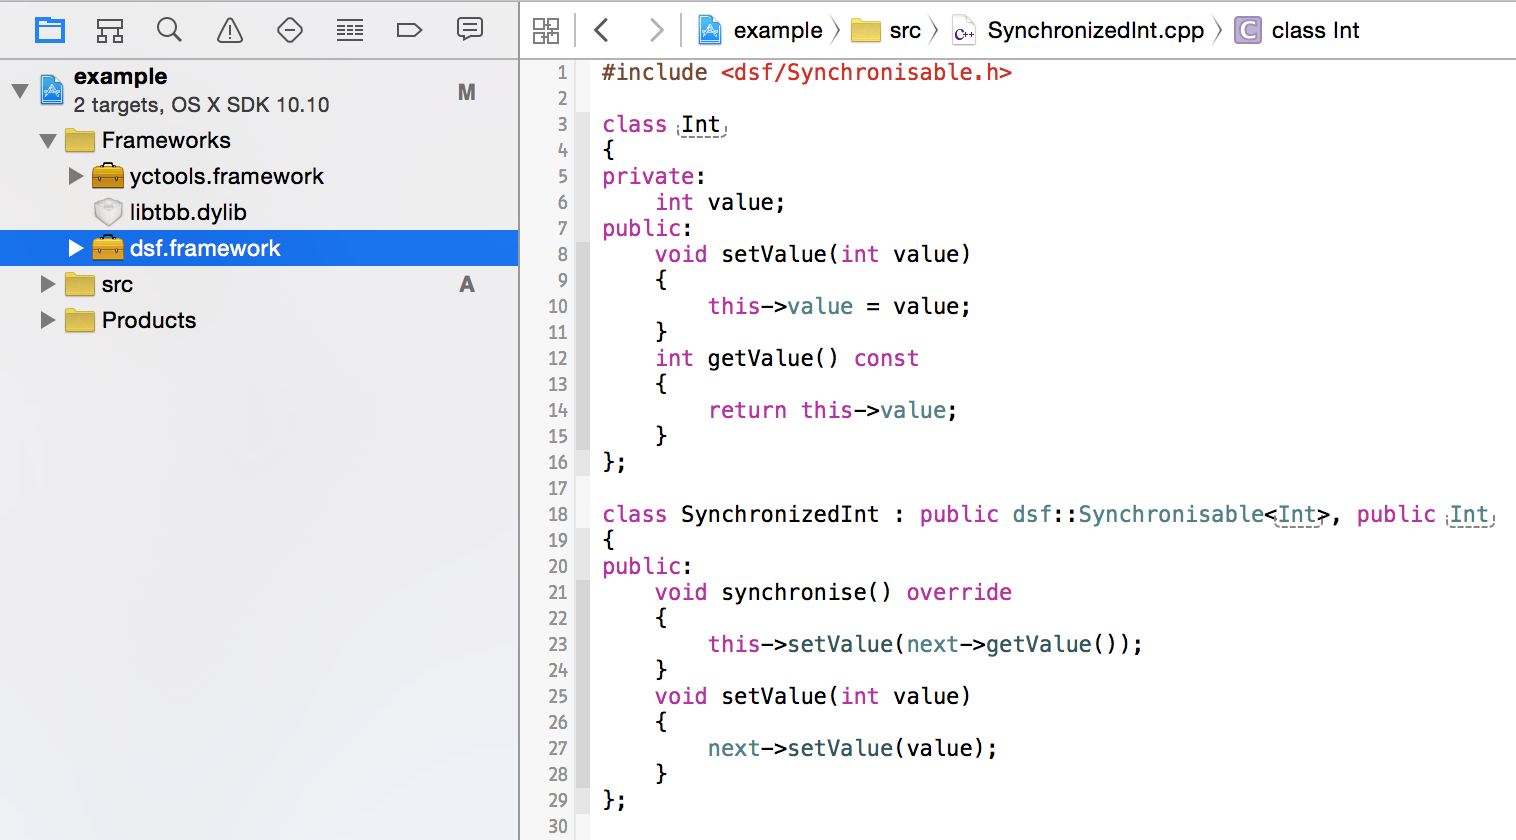
\includegraphics[width=\textwidth,height=\textheight/2,keepaspectratio=true]{ReportDescriptionXcode.png}}
\end{DoxyImageNoCaption}
\hypertarget{_project_description_ProjectDescriptionBenchmarkProgram}{}\section{Benchmark Program}\label{_project_description_ProjectDescriptionBenchmarkProgram}
The benchmark program is designed for profiling the library. It allows user to configure settings. 
\begin{DoxyImageNoCaption}
  \mbox{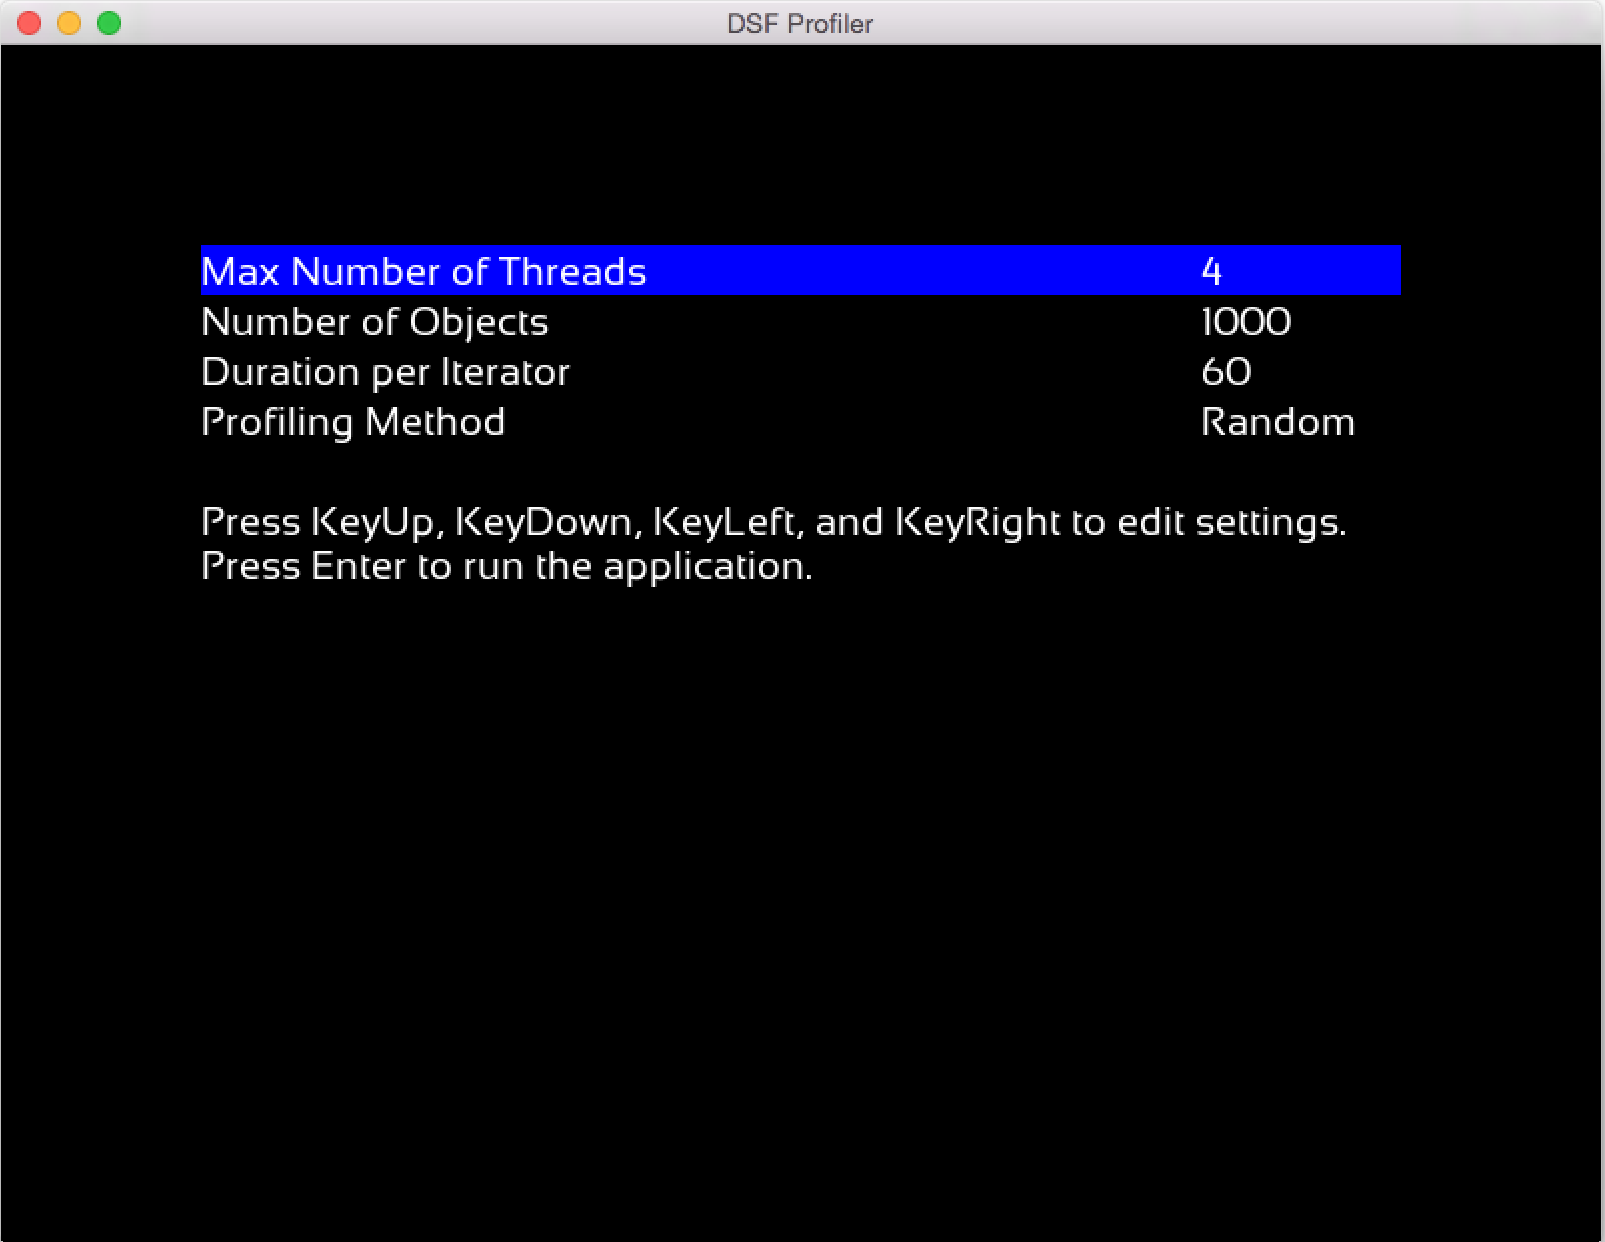
\includegraphics[width=12cm]{ReportDescriptionBenchmark.png}}
\end{DoxyImageNoCaption}
 While running it shows the maximum, minimum, and average F\+P\+S on the screen. 
\begin{DoxyImageNoCaption}
  \mbox{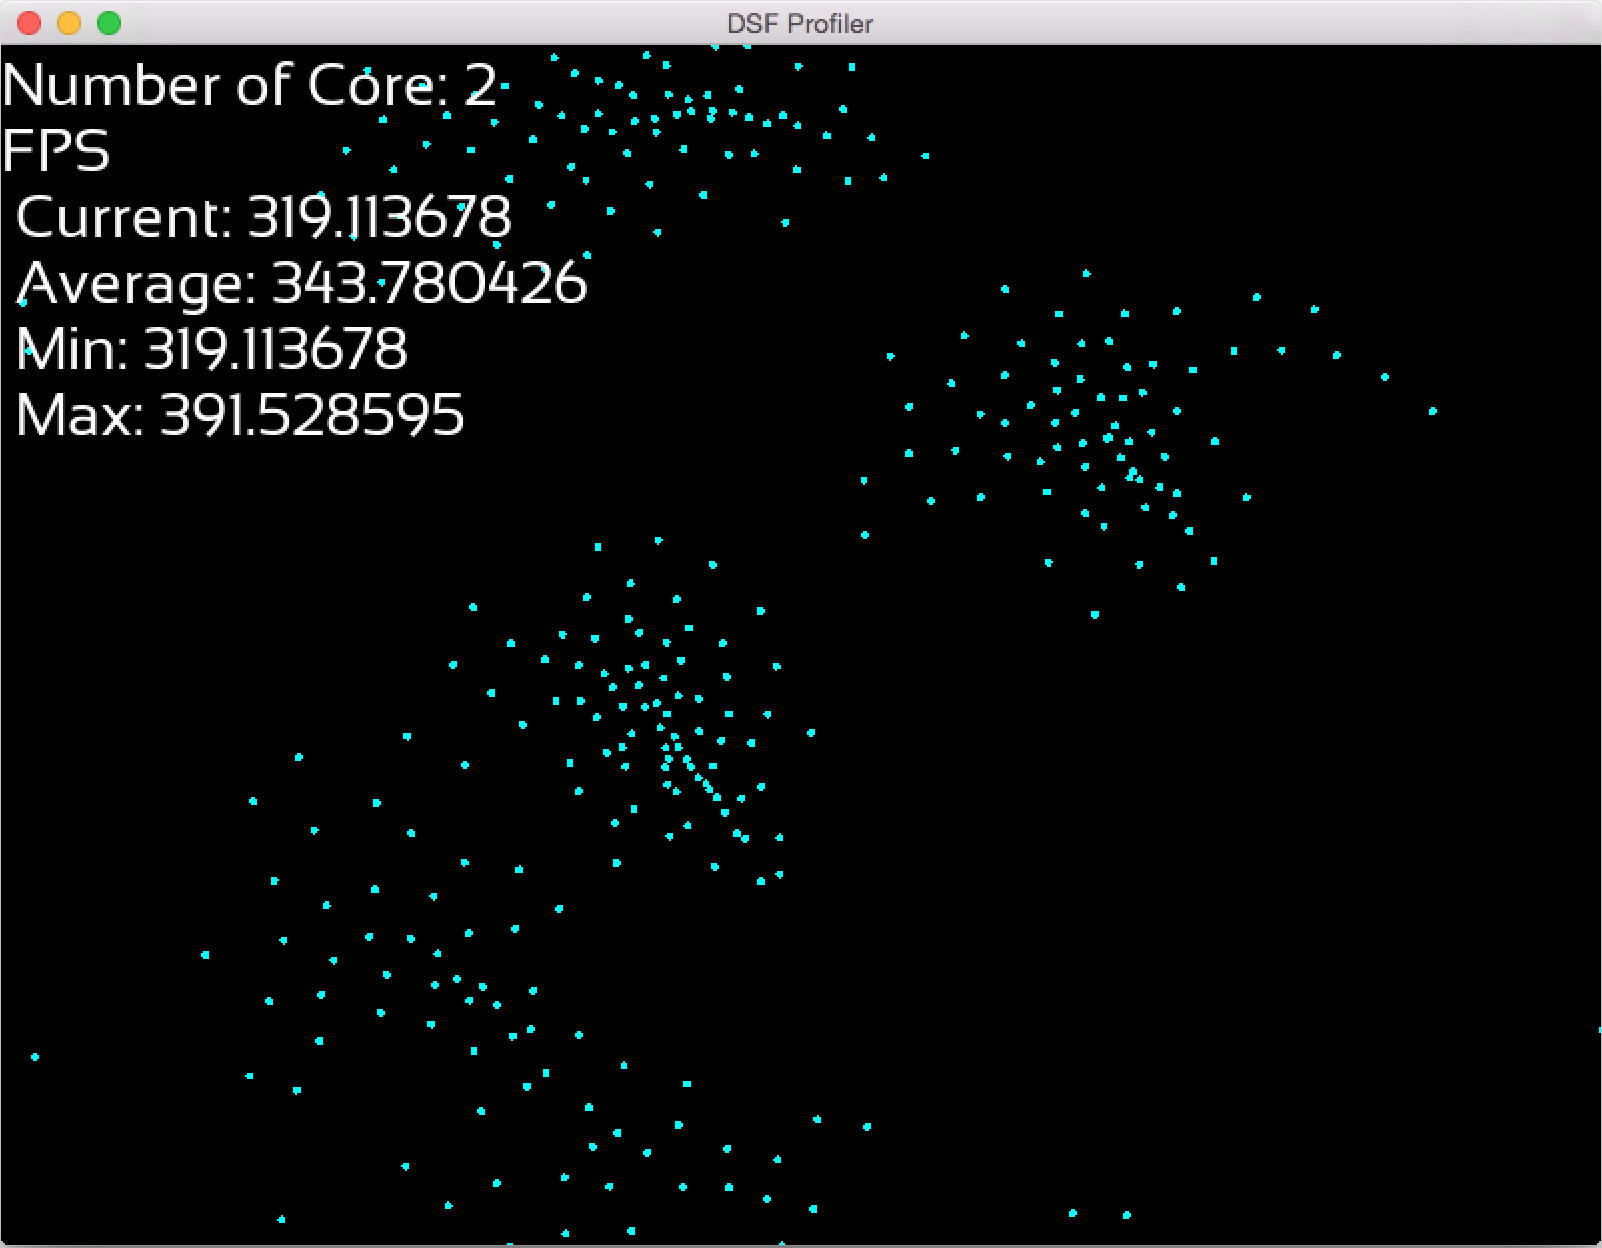
\includegraphics[width=12cm]{ReportDescriptionBenchmarkRunning.png}}
\end{DoxyImageNoCaption}
 The output is a bar graph. X axis is the number of threads, and y axis in the F\+P\+S. 
\begin{DoxyImageNoCaption}
  \mbox{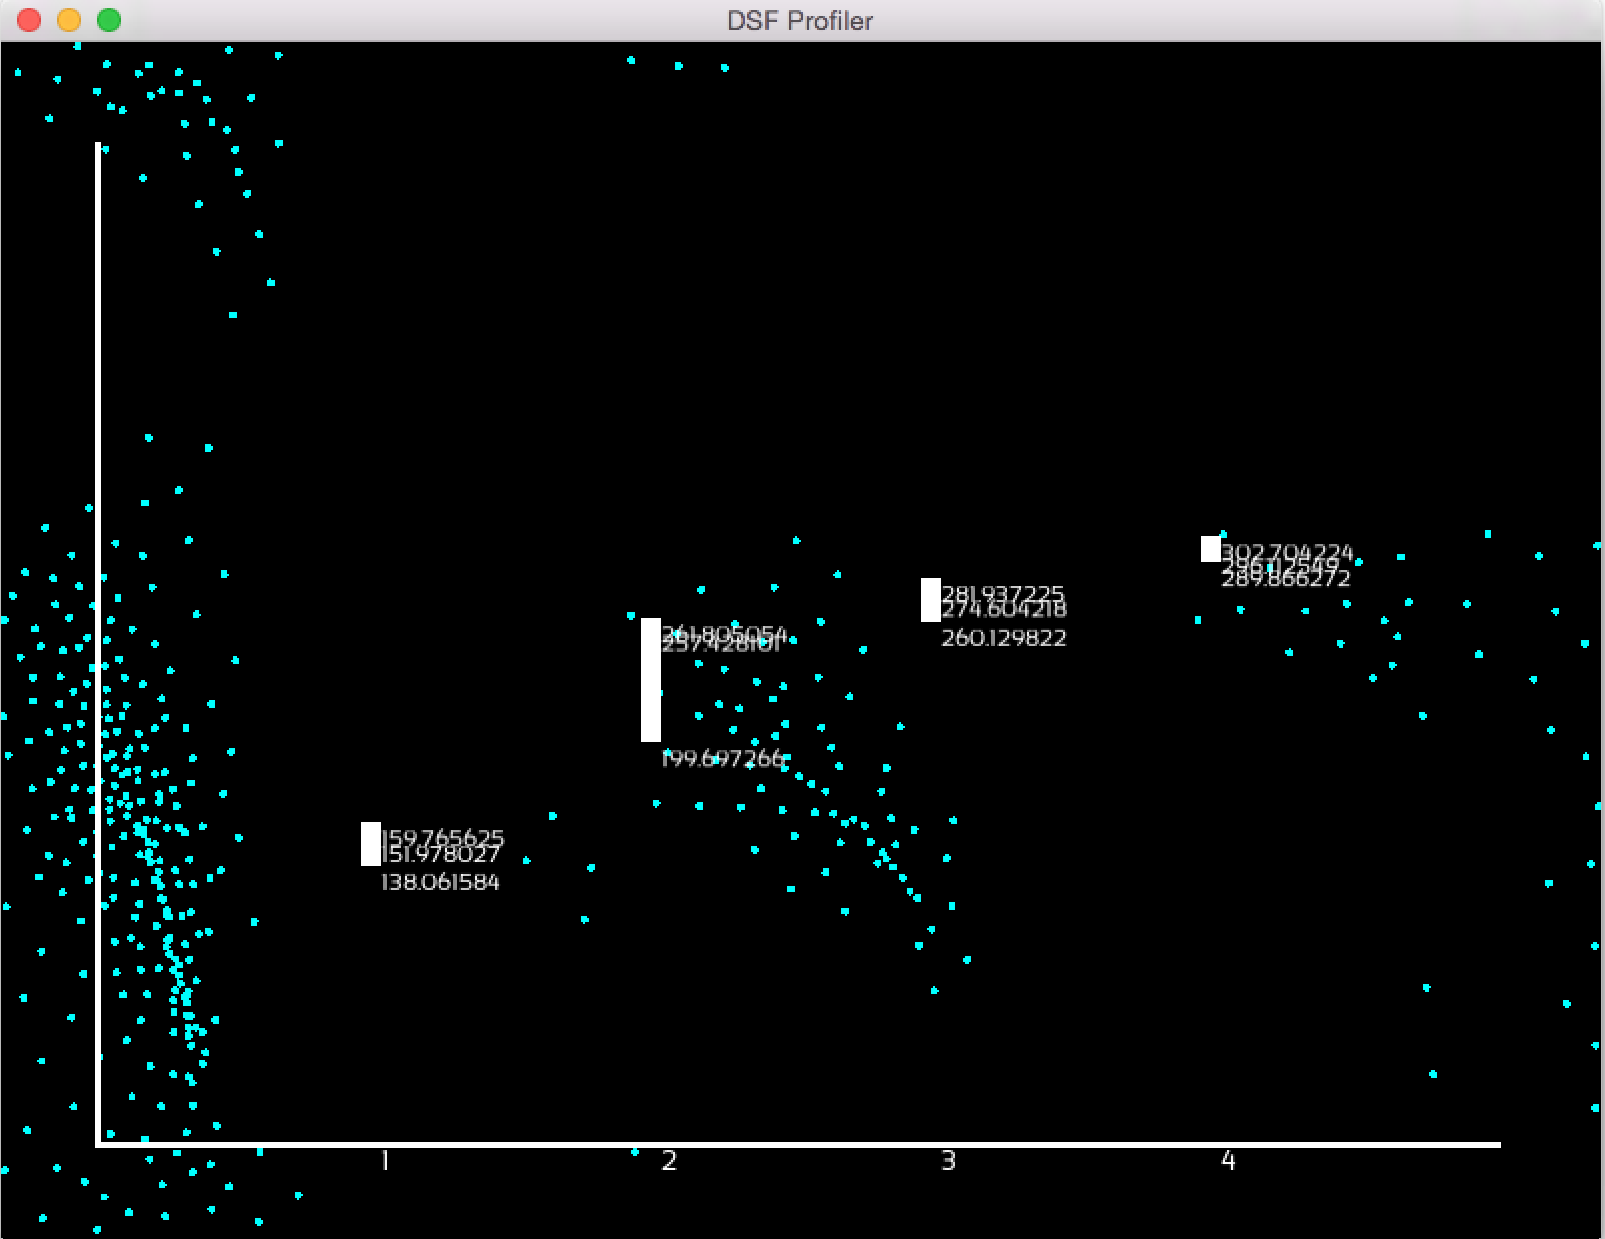
\includegraphics[width=12cm]{ReportDescriptionBenchmarkOutput.png}}
\end{DoxyImageNoCaption}
 
\chapter{Conformance to Specification and Design Manual}
\label{_conformanceto_specificationand_design_manual}
\hypertarget{_conformanceto_specificationand_design_manual}{}
Fortunately, the submitted product matches all functionalities that my specification and design documents mentioned. \hypertarget{_conformanceto_specificationand_design_manual_SetupDevelopmentEnvironment}{}\section{Setup Development Environment}\label{_conformanceto_specificationand_design_manual_SetupDevelopmentEnvironment}
The operating system of my laptop is Mac O\+S X Yosemite \cite{osxyosemite}. I have installed V\+Mware Fusion \cite{vmwarefusion} and have created two virtual machine for other operating systems(Microsoft Windows 7 \cite{microsoftwindows7} and Ubuntu 14.\+04 L\+T\+S \cite{ubuntu14_04LTS}). The development will be mainly taken place under Mac, and tested in all these three operating systems. \hypertarget{_conformanceto_specificationand_design_manual_SetupDevelopmentEnvironmentCppCompilerandIDE}{}\subsection{C++ Compiler and I\+D\+E}\label{_conformanceto_specificationand_design_manual_SetupDevelopmentEnvironmentCppCompilerandIDE}
\begin{DoxyParagraph}{Mac O\+S X}
To setup Xcode \cite{xcode} and default C++ compiler L\+L\+V\+M \cite{llvm} in Mac O\+S X is very easy.
\begin{DoxyItemize}
\item Open App Store → search \char`\"{}\+Xcode\char`\"{} → click \char`\"{}get\char`\"{} button
\end{DoxyItemize}
\end{DoxyParagraph}
After the installation, the I\+D\+E Xcode and the compiler L\+L\+V\+M is installed. To see the information about clang by command \char`\"{}clang -\/-\/version\char`\"{}. 
\begin{DoxyCode}
MacBook-Pro:~ yuchen$ clang --version
Apple LLVM version 6.1.0 (clang-602.0.49) (based on LLVM 3.6.0svn)
Target: x86\_64-apple-darwin14.3.0
\end{DoxyCode}
 \begin{DoxyParagraph}{Microsoft Windows}
Download Visual Studio Community \cite{visualstudiocommunity} from \href{https://www.visualstudio.com}{\tt https\+://www.\+visualstudio.\+com} and install it. Visual Studio has its own embedded C++ compiler. 
\end{DoxyParagraph}
\begin{DoxyParagraph}{Ubuntu}
Open a terminal and type following command to install the G\+N\+U Compiler Collection(\+G\+C\+C) \cite{gcc} 
\begin{DoxyCode}
sudo apt-\textcolor{keyword}{get} install build-essential
\end{DoxyCode}
 Type \char`\"{}gcc -\/v\char`\"{} to print the descriptions. 
\begin{DoxyCode}
yu@ubuntu:~$ gcc -v
Using built-in specs.
COLLECT\_GCC=gcc
COLLECT\_LTO\_WRAPPER=/usr/lib/gcc/x86\_64-linux-gnu/4.8/lto-wrapper
Target: x86\_64-linux-gnu
Configured with: ../src/configure -v --with-pkgversion=\textcolor{stringliteral}{'Ubuntu 4.8.2-19ubuntu1'} --with-bugurl=file:
Thread model: posix
gcc version 4.8.2 (Ubuntu 4.8.2-19ubuntu1) 
\end{DoxyCode}

\end{DoxyParagraph}
\hypertarget{_conformanceto_specificationand_design_manual_SetupDevelopmentEnvironmentThirdpartylibraries}{}\subsection{Third party libraries}\label{_conformanceto_specificationand_design_manual_SetupDevelopmentEnvironmentThirdpartylibraries}
\begin{DoxyParagraph}{Intel Threading Building Blocks}
Intel T\+B\+B \cite{inteltbb} is a C++ library for parallel computing. Use Homebrew \cite{homebrew} to Install the library for Mac O\+S X\+: 
\begin{DoxyCode}
$ brew install libtbb
\end{DoxyCode}
 For Ubuntu use following command 
\begin{DoxyCode}
$ sudo apt-\textcolor{keyword}{get} install libtbb2
\end{DoxyCode}
 For Window need go to its download page \href{https://www.threadingbuildingblocks.org/download}{\tt https\+://www.\+threadingbuildingblocks.\+org/download}. Download the Windows version binaries package and unzip it.
\begin{DoxyItemize}
\item First, create a a new folder. The full path of it is \char`\"{}\+C\+:\textbackslash{}\+Program Files\textbackslash{}tbb\char`\"{}. Inside the folder create three folders \char`\"{}include\char`\"{}, \char`\"{}lib\char`\"{}, and \char`\"{}bin\char`\"{}.
\item Secondly, go to the unzipped folder. Copy everything inside the \char`\"{}include\char`\"{} to the \char`\"{}include\char`\"{} has just been created.
\item Inside the \char`\"{}lib\char`\"{}, there are two folders \char`\"{}ia32\char`\"{} and \char`\"{}intel64\char`\"{} that means the architecture of operating system. My Window 7 is 32 bits, so I chose the \char`\"{}ia32\char`\"{}. Again, inside \char`\"{}ia32\char`\"{}, there are many folders those are the versions of Visual Studio. The version of Visual Studio that I installed is 2013. The core of Visual Studio 2013 is vs2012, so copy all files inside \char`\"{}vc12\char`\"{} to the folder \char`\"{}lib\char`\"{} which has just been created.
\item Inside the \char`\"{}bin\char`\"{}, do the same thing as \char`\"{}lib\char`\"{} did.
\item Create a environment variable \char`\"{}tbb\char`\"{} refers to the directory \char`\"{}\+C\+:\textbackslash{}\+Program Files\textbackslash{}tbb\char`\"{}.
\end{DoxyItemize}
\end{DoxyParagraph}
\begin{DoxyParagraph}{S\+F\+M\+L}
Simple and Fast Multimedia Library(S\+F\+M\+L \cite{sfml}) is a graphics library. For Mac, just go to the download page \href{http://www.sfml-dev.org/download/sfml/2.1/}{\tt http\+://www.\+sfml-\/dev.\+org/download/sfml/2.\+1/} to get the installer and run it. For Ubuntu, just need one line command\+: 
\begin{DoxyCode}
sudo apt-\textcolor{keyword}{get} install libsfml-dev
\end{DoxyCode}
 However, there is a problem for Windows. When I went to its download page, I could not find the version for Visual Studio 2013. The solution is to compile the source code which can be cloned from \href{https://github.com/LaurentGomila/SFML.git}{\tt https\+://github.\+com/\+Laurent\+Gomila/\+S\+F\+M\+L.\+git}.
\end{DoxyParagraph}
\hypertarget{_conformanceto_specificationand_design_manual_SetupDevelopmentEnvironmentOtherTools}{}\subsection{Other Tools}\label{_conformanceto_specificationand_design_manual_SetupDevelopmentEnvironmentOtherTools}

\begin{DoxyItemize}
\item Source\+Tree \cite{sourcetree}, a G\+U\+I git front-\/end, which is available in both Mac and Windows.
\item cmake-\/gui \cite{cmakegui}, the official G\+U\+I front-\/end for C\+Make, available in Mac, Windows, and Linux.
\end{DoxyItemize}\hypertarget{_conformanceto_specificationand_design_manual_StartDevelopment}{}\section{Start Development}\label{_conformanceto_specificationand_design_manual_StartDevelopment}
\hypertarget{_conformanceto_specificationand_design_manual_StartDevelopmentSourceControl}{}\subsection{Source Control}\label{_conformanceto_specificationand_design_manual_StartDevelopmentSourceControl}
I used git for source control. The repository is available at \href{https://github.com/kuyoonjo/DualStateFramework.git}{\tt https\+://github.\+com/kuyoonjo/\+Dual\+State\+Framework.\+git}. \hypertarget{_conformanceto_specificationand_design_manual_StartDevelopmentCodeConfigurations}{}\subsection{Code Configurations}\label{_conformanceto_specificationand_design_manual_StartDevelopmentCodeConfigurations}
The project is designed for Mac O\+S X, Microsoft Window, and other Unix-\/like operating systems. Therefore, the code should be portable in all of them. Write different copy for different operating system is not a good idea. The best solution is prepare some configuration file, then different operating system will generate different copies. \begin{DoxyParagraph}{Config.h}

\begin{DoxyCode}
\textcolor{preprocessor}{#ifndef dsf\_Config\_h}
\textcolor{preprocessor}{#define dsf\_Config\_h}

\textcolor{preprocessor}{#if defined(\_WIN32)}

\textcolor{comment}{// Windows compilers need specific (and different) keywords for export and import}
\textcolor{preprocessor}{#define DSF\_API\_EXPORT \_\_declspec(dllexport)}
\textcolor{preprocessor}{#define DSF\_API\_IMPORT \_\_declspec(dllimport)}

\textcolor{comment}{// For Visual C++ compilers, we also need to turn off this annoying C4251 warning}
\textcolor{preprocessor}{#ifdef \_MSC\_VER}

\textcolor{preprocessor}{#pragma warning(disable : 4251)}

\textcolor{preprocessor}{#endif}

\textcolor{preprocessor}{#else // Linux, FreeBSD, Mac OS X}

\textcolor{preprocessor}{#if \_\_GNUC\_\_ >= 4}

\textcolor{comment}{// GCC 4 has special keywords for showing/hidding symbols,}
\textcolor{comment}{// the same keyword is used for both importing and exporting}
\textcolor{preprocessor}{#define DSF\_API\_EXPORT \_\_attribute\_\_ ((\_\_visibility\_\_ ("default")))}
\textcolor{preprocessor}{#define DSF\_API\_IMPORT \_\_attribute\_\_ ((\_\_visibility\_\_ ("default")))}

\textcolor{preprocessor}{#else}

\textcolor{comment}{// GCC < 4 has no mechanism to explicitely hide symbols, everything's exported}
\textcolor{preprocessor}{#define DSF\_API\_EXPORT}
\textcolor{preprocessor}{#define DSF\_API\_IMPORT}

\textcolor{preprocessor}{#endif}

\textcolor{preprocessor}{#endif}


\textcolor{preprocessor}{#endif}
\end{DoxyCode}
 
\end{DoxyParagraph}
\begin{DoxyParagraph}{Export.h}

\begin{DoxyCode}
\textcolor{preprocessor}{#ifndef dsf\_Export\_h}
\textcolor{preprocessor}{#define dsf\_Export\_h}

\textcolor{comment}{// Headers}
\textcolor{comment}{}\textcolor{preprocessor}{#include "Config.h"}


\textcolor{comment}{// Define portable import / export macros}
\textcolor{comment}{}\textcolor{preprocessor}{#if defined(dsf\_EXPORTS)}

\textcolor{preprocessor}{#define DSF\_API DSF\_API\_EXPORT}

\textcolor{preprocessor}{#else}

\textcolor{preprocessor}{#define DSF\_API DSF\_API\_IMPORT}

\textcolor{preprocessor}{#endif}

\textcolor{preprocessor}{#endif}
\end{DoxyCode}

\end{DoxyParagraph}
\hypertarget{_conformanceto_specificationand_design_manual_StartDevelopmentBuildProcessManagement}{}\subsection{Build Process Management}\label{_conformanceto_specificationand_design_manual_StartDevelopmentBuildProcessManagement}
Different I\+D\+Es use different build process managements.
\begin{DoxyItemize}
\item A bundle with extension name \char`\"{}xcodeproj\char`\"{} is an Xcode project.
\item A file with extension name \char`\"{}sln\char`\"{} is a Visual Studio Solution.
\item G\+C\+C uses Makefile.
\item Many others.
\end{DoxyItemize}

C\+Make can generate different build process systems for those. What I need is a little bit configurations for different I\+D\+Es. 
\begin{DoxyCode}
\textcolor{keywordflow}{if} (MSVC)
\textcolor{preprocessor}{    # Windows VC}
\textcolor{preprocessor}{    # Activate C++ exception handling}
    \textcolor{keywordflow}{if} (NOT CMAKE\_CXX\_FLAGS MATCHES \textcolor{stringliteral}{"/EHsc"})
    set(CMAKE\_CXX\_FLAGS \textcolor{stringliteral}{"$\{CMAKE\_CXX\_FLAGS\} /EHsc"})
    endif ()

    \textcolor{preprocessor}{# Set Warning level always to 4}
    \textcolor{keywordflow}{if} (CMAKE\_CXX\_FLAGS MATCHES \textcolor{stringliteral}{"/W[0-4]"})
        string(REGEX REPLACE \textcolor{stringliteral}{"/W[0-4]"} \textcolor{stringliteral}{"/W4"} CMAKE\_CXX\_FLAGS \textcolor{stringliteral}{"$\{CMAKE\_CXX\_FLAGS\}"})
    \textcolor{keywordflow}{else} ()
        set(CMAKE\_CXX\_FLAGS \textcolor{stringliteral}{"$\{CMAKE\_CXX\_FLAGS\} /W4"})
    endif () 
elseif(APPLE)
    \textcolor{preprocessor}{# Mac OS X Xcode}
    set(CMAKE\_MACOSX\_RPATH 1)
    ADD\_DEFINITIONS(-std=c++11)
else()
    \textcolor{preprocessor}{# Unix}
    ADD\_DEFINITIONS(-std=c++11)
endif()
\end{DoxyCode}
\hypertarget{_conformanceto_specificationand_design_manual_Implementation}{}\section{Implementation}\label{_conformanceto_specificationand_design_manual_Implementation}
\hypertarget{_conformanceto_specificationand_design_manual_ImplementationDualState}{}\subsection{Dual State}\label{_conformanceto_specificationand_design_manual_ImplementationDualState}
The idea to make an object two states is to create an abstract class named \char`\"{}\+Synchronisable\char`\"{} that any other class inherits it will have two copies. The class is designed as this\+: 
\begin{DoxyCode}
\textcolor{keyword}{template}<\textcolor{keyword}{class} T> \textcolor{keyword}{class }Synchronisable
\{
\textcolor{keyword}{protected}:
    T* next; \textcolor{comment}{//A copy of current object.}
\textcolor{keyword}{public}:
    \textcolor{keyword}{virtual} ~Synchronisable() \{
        \textcolor{keyword}{delete} this->next;
    \}
    \textcolor{keyword}{virtual} \textcolor{keywordtype}{void} synchronise() = 0; \textcolor{comment}{//Signs current value to next value.}
\};
\end{DoxyCode}
 Any class implements the abstract class will automatically generate a copy \char`\"{}next\char`\"{} when an object is created. What we need to do is just override the method \char`\"{}synchronise\char`\"{}. For example\+: 
\begin{DoxyCode}
\textcolor{preprocessor}{#include <dsf/Synchronisable.h>}

\textcolor{keyword}{class }Int
\{
\textcolor{keyword}{private}:
    \textcolor{keywordtype}{int} value;
\textcolor{keyword}{public}:
    \textcolor{keywordtype}{void} setValue(\textcolor{keywordtype}{int} value)
    \{
        this->value = value;
    \}
    \textcolor{keywordtype}{int} getValue()\textcolor{keyword}{ const}
\textcolor{keyword}{    }\{
        \textcolor{keywordflow}{return} this->value;
    \}
\};

\textcolor{keyword}{class }SynchronizedInt : \textcolor{keyword}{public} dsf::Synchronisable<Int>, \textcolor{keyword}{public} Int
\{
\textcolor{keyword}{public}:
    \textcolor{keywordtype}{void} synchronise()\textcolor{keyword}{ override}
\textcolor{keyword}{    }\{
        this->setValue(next->getValue());
    \}
\};
\end{DoxyCode}
\hypertarget{_conformanceto_specificationand_design_manual_Implementationrnd}{}\subsection{Read operation and Write operation}\label{_conformanceto_specificationand_design_manual_Implementationrnd}
Now, we need to make the current value for all read operations, and the next value for all write operations. To implement this, we just need to override the method \char`\"{}set\+Value\char`\"{}. 
\begin{DoxyCode}
\textcolor{keywordtype}{void} setValue(\textcolor{keywordtype}{int} value)
\{
    next->setValue(value);
\}
\end{DoxyCode}
 Every time we call the method \char`\"{}set\+Value\char`\"{} will effect the next, but not the current. The example code will now like this\+: 
\begin{DoxyCodeInclude}
\textcolor{preprocessor}{#include <dsf/Synchronisable.h>}

\textcolor{keyword}{class }Int
\{
\textcolor{keyword}{private}:
    \textcolor{keywordtype}{int} value;
\textcolor{keyword}{public}:
    \textcolor{keywordtype}{void} setValue(\textcolor{keywordtype}{int} value)
    \{
        this->value = value;
    \}
    \textcolor{keywordtype}{int} getValue()\textcolor{keyword}{ const}
\textcolor{keyword}{    }\{
        \textcolor{keywordflow}{return} this->value;
    \}
\};

\textcolor{keyword}{class }SynchronizedInt : \textcolor{keyword}{public} dsf::Synchronisable<Int>, \textcolor{keyword}{public} Int
\{
\textcolor{keyword}{public}:
    \textcolor{keywordtype}{void} synchronise()\textcolor{keyword}{ override}
\textcolor{keyword}{    }\{
        this->setValue(next->getValue());
    \}
    \textcolor{keywordtype}{void} setValue(\textcolor{keywordtype}{int} value)
    \{
        next->setValue(value);
    \}
\};
\end{DoxyCodeInclude}
\hypertarget{_conformanceto_specificationand_design_manual_ImplementationBenchmarkProgram}{}\subsection{Benchmark Program}\label{_conformanceto_specificationand_design_manual_ImplementationBenchmarkProgram}
For benchmarks, I used S\+F\+M\+L to create graphics. Frames per Second is the measurement for the benchmark program. Three methods of different algorithms are used\+:
\begin{DoxyItemize}
\item Random
\item Elastic collision
\item Flocking boids
\end{DoxyItemize}

Because of S\+F\+M\+L using opengl, and opengl not supporting multiple-\/thread rendering, the step of draw elements should be in serial programming phase. A class was designed for S\+F\+M\+L\+: 
\begin{DoxyCodeInclude}
\textcolor{comment}{//}
\textcolor{comment}{//  DSFSFML.h}
\textcolor{comment}{//  profiler}
\textcolor{comment}{//}
\textcolor{comment}{//  Created by Yu Chen on 2/16/15.}
\textcolor{comment}{//}
\textcolor{comment}{//}

\textcolor{preprocessor}{#ifndef profiler\_DSFSFML\_h}
\textcolor{preprocessor}{#define profiler\_DSFSFML\_h}

\textcolor{preprocessor}{#include <SFML/Graphics.hpp>}
\textcolor{preprocessor}{#include <vector>}

\textcolor{keyword}{namespace }dsf
\{
    \textcolor{keyword}{namespace }sfml
    \{
        \textcolor{keyword}{class }RenderWindow
        \{
        \textcolor{keyword}{public}:
            \textcolor{keyword}{explicit} RenderWindow();
            \textcolor{keyword}{virtual} ~RenderWindow();
            sf::RenderWindow* window;
            std::vector<sf::Drawable*>* drawables;
        \textcolor{keyword}{protected}:
            \textcolor{keyword}{virtual} \textcolor{keywordtype}{void} draw() = 0;
        \};
    \}
\}
\textcolor{preprocessor}{#endif}
\end{DoxyCodeInclude}
 In parallel programming phase, all elements need to be drawn will be pushed in to the list drawables. In serial phase, all elements in the list will be drawn out. 
\chapter{Description of Learning}
\label{_descriptionof_learning}
\hypertarget{_descriptionof_learning}{}
\hypertarget{_descriptionof_learning_DescriptionofLearningTechnical}{}\section{Technical}\label{_descriptionof_learning_DescriptionofLearningTechnical}
By developing this framework I learned a lot of information\+:
\begin{DoxyItemize}
\item Dynamic-\/link library.
\begin{DoxyItemize}
\item how dynamic-\/link works on different operating systems
\item export symbols and import symbols
\end{DoxyItemize}
\item Intel T\+B\+B
\begin{DoxyItemize}
\item how Intel T\+B\+B implements parallel programming
\item how to execute a program by a specified number of threads
\end{DoxyItemize}
\item C++11 features
\begin{DoxyItemize}
\item when and how to use smart pointers
\item function pointers and Lambdas
\item override and final keywords
\end{DoxyItemize}
\item Mac os X related
\begin{DoxyItemize}
\item Mac library bundle
\item Mac application bundle
\item @rpath, @excutable\+\_\+path, and @load\+\_\+path
\item how to use otool command to display specified parts of object files or libraries
\item how to use install\+\_\+name\+\_\+tool command to edit specified parts of object files or libraries
\end{DoxyItemize}
\item Algorithms
\begin{DoxyItemize}
\item Elastic collision
\item Flocking Boids
\end{DoxyItemize}
\item C\+Make
\begin{DoxyItemize}
\item how to create a Mac bundle, and copy relative files to the bundle
\item how to detect a specified library is installed or not
\item how to add extra headings and libraries
\end{DoxyItemize}
\item Others
\begin{DoxyItemize}
\item how to use Doxygen to generate La\+Tex format documents
\item how to use Graphviz and D\+O\+T to create inheritance diagrams
\item how to use La\+Tex to create pdf documents.
\item how to use Bib\+Te\+X to manage bibliography.
\end{DoxyItemize}
\end{DoxyItemize}\hypertarget{_descriptionof_learning_DescriptionofLearningPersonal}{}\section{Personal}\label{_descriptionof_learning_DescriptionofLearningPersonal}
I did not practice good Time management and Project management skills during the most of project development. As a result of this project work, I have once more realized that the Time management and Project management are important personal skills, which should be always improved. Also, I have achieved presentation skills through project presentations and demos. 
\chapter{Review of Project}
\label{_reviewof_project}
\hypertarget{_reviewof_project}{}
Overall, the project went very smoothly. One of the things I was very happy with was the fact that the benchmark program gave me a surprise. Before the benchmarks, I thought that if the number of threads increases, then the F\+P\+S will grow proportionally. However, the result depends on the C\+P\+U. For example, my C\+P\+U is Intel i5 with 2 cores running 4 threads. The best performance is using 4 threads to run the framework.\hypertarget{_reviewof_project_ReviewofProjectPEF}{}\section{Problems Encountered \& Fixes}\label{_reviewof_project_ReviewofProjectPEF}
\hypertarget{_reviewof_project_ReviewofProjectPEFMemoryLeaks}{}\subsection{Memory Leaks}\label{_reviewof_project_ReviewofProjectPEFMemoryLeaks}
\begin{DoxyParagraph}{Background}
I tries to implement a class type that can be signed as any type of value like this\+: 
\begin{DoxyCode}
Any one = int(1);
Any pi = float(3.14);
Any rect = Rectangle(2, 3);
\end{DoxyCode}
 Originally, I used void pointer to save the value. 
\begin{DoxyCode}
\textcolor{keyword}{class }Any
\{
\textcolor{keyword}{private}:
    \textcolor{keywordtype}{void}* value;
\}
\end{DoxyCode}
 
\end{DoxyParagraph}
\begin{DoxyParagraph}{Reason}
When I ran the code, there was a memory leak issue. The reason is that a void pointer cannot be released. 
\begin{DoxyCode}
\textcolor{keywordtype}{void}* i = \textcolor{keyword}{new} int() \textcolor{comment}{// no problem}
delete i; \textcolor{comment}{// it will not deallocate the memory}
\end{DoxyCode}
 
\end{DoxyParagraph}
\begin{DoxyParagraph}{Solution}
I could cast the pointer to a specified type and delete it. 
\begin{DoxyCode}
\textcolor{keywordtype}{void}* i = \textcolor{keyword}{new} int() \textcolor{comment}{// no problem}
delete (\textcolor{keywordtype}{int})i; \textcolor{comment}{// works fine}
\end{DoxyCode}
 However, if I did that way, the class Any should be designed as a template class. That would be meaningless. The solution was using smart pointer indeed of traditional pointer.
\end{DoxyParagraph}
\hypertarget{_reviewof_project_ReviewofProjectPEFWrongPathwithDynamiclinkLibrary}{}\subsection{Wrong path with dynamic-\/link library}\label{_reviewof_project_ReviewofProjectPEFWrongPathwithDynamiclinkLibrary}
\begin{DoxyParagraph}{Background}
When I tried to package resources to an App bundle, I got an error message\+: 
\begin{DoxyCode}
dyld: Library not loaded: libtbb.dylib
  Referenced from: /Users/yuchen/Documents/XCode/profiler/build/Release/profiler.app/Contents/MacOS/
      profiler
  Reason: image not found
\end{DoxyCode}
 
\end{DoxyParagraph}
\begin{DoxyParagraph}{Reason}
Mac App Bundle uses @rpath, @excutable\+\_\+path, and @load\+\_\+path to handle the resource path. By using otool command, I got the message as below\+: 
\begin{DoxyCode}
MacBook-Pro:libs-osx yuchen$ otool -L libtbb.dylib 
libtbb.dylib:
    libtbb.dylib (compatibility version 0.0.0, current version 0.0.0)
    /usr/lib/libSystem.B.dylib (compatibility version 1.0.0, current version 1197.1.1)
    mac64/libcilkrts.5.dylib (compatibility version 0.0.0, current version 0.0.0)
    /usr/lib/libstdc++.6.dylib (compatibility version 7.0.0, current version 60.0.0)
    /usr/lib/libgcc\_s.1.dylib (compatibility version 1.0.0, current version 2577.0.0)
\end{DoxyCode}
 The third line is the reference path for the dynamic-\/link library. 
\end{DoxyParagraph}
\begin{DoxyParagraph}{Solution}
The solution was using install\+\_\+name\+\_\+tool command to change the reference path. 
\begin{DoxyCode}
MacBook-Pro:libs-osx yuchen$ install\_name\_tool -\textcolor{keywordtype}{id} @executable\_path/../Frameworks/libtbb.dylib libtbb.dylib
       
MacBook-Pro:libs-osx yuchen$ otool -L libtbb.dylib 
libtbb.dylib:
    @executable\_path/../Frameworks/libtbb.dylib (compatibility version 0.0.0, current version 0.0.0)
    /usr/lib/libSystem.B.dylib (compatibility version 1.0.0, current version 1197.1.1)
    mac64/libcilkrts.5.dylib (compatibility version 0.0.0, current version 0.0.0)
    /usr/lib/libstdc++.6.dylib (compatibility version 7.0.0, current version 60.0.0)
    /usr/lib/libgcc\_s.1.dylib (compatibility version 1.0.0, current version 2577.0.0)
\end{DoxyCode}

\end{DoxyParagraph}
\hypertarget{_reviewof_project_ReviewofProjectPEFSomefunctionsandvariablesnotdefined}{}\subsection{Some functions and variables not defined}\label{_reviewof_project_ReviewofProjectPEFSomefunctionsandvariablesnotdefined}
\begin{DoxyParagraph}{Background}
I used C++ std library for this project. It worked fine in Mac O\+S X. However, when I debugged it in Windows and Linux, some error message prompted out. 
\begin{DoxyCode}
Error   3   error C2065: \textcolor{stringliteral}{'M\_PI'} : undeclared identifier C:
      \(\backslash\)Users\(\backslash\)Administrator\(\backslash\)Documents\(\backslash\)DualStateFramework\(\backslash\)profiler\(\backslash\)src\(\backslash\)BouncingCircleManager.cpp  104 1   profiler
\end{DoxyCode}
 
\end{DoxyParagraph}
\begin{DoxyParagraph}{Reason}
The reason is that M\+\_\+\+P\+I is not \char`\"{}pure\char`\"{} standard. Most compilers regard it as a standard, but Visual C++ not. The similar problem I met is G\+C\+C does not know what std\+::powf is, but both L\+L\+V\+M and Visual C++ use it as a standard. 
\end{DoxyParagraph}
\begin{DoxyParagraph}{Solution}
Once I knew the reason, the solution was easily made up. For M\+\_\+\+P\+I, I added a preprocessor definition \+\_\+\+U\+S\+E\+\_\+\+M\+A\+T\+H\+\_\+\+D\+E\+F\+I\+N\+E\+S for Visual Studio by C\+Make\+List\+: 
\begin{DoxyCode}
\textcolor{preprocessor}{# Add Math definitions}
\textcolor{preprocessor}{add\_definitions(-D\_USE\_MATH\_DEFINES)}
\end{DoxyCode}
 For std\+::powf, I changed it to std\+::pow, which is the standard. 
\end{DoxyParagraph}
\hypertarget{_reviewof_project_ReviewofProjectAttemptingtheProjectAgain}{}\section{Attempting the Project Again}\label{_reviewof_project_ReviewofProjectAttemptingtheProjectAgain}
If I were to attempt the project again I would avoid using pointers if they are not necessary. I think this is because my first Object Oriented Programming language is Java. In Java word, all objects should be created by keyword \char`\"{}new\char`\"{}. However, that is not guaranteed in C++. The reason is Java virtual machine has garbage collection but C++ not, which means in C++, objects created by \char`\"{}new\char`\"{} need user to deallocate them manually. ~\newline
~\newline
Pointers sometimes make users confused in a framework. For example, in this framework, some pointers passed by functions will be deleted automatically. 
\begin{DoxyCode}
\textcolor{keywordtype}{void} send(SynchronizedObject* to,
          TaskFunction* taskFunction,
          TaskArgument* args);
\end{DoxyCode}
 The method \char`\"{}send\char`\"{} takes three pointers as arguments. The third one \char`\"{}args\char`\"{} will be deleted automatically, but \char`\"{}task\+Function\char`\"{} or \char`\"{}to\char`\"{} not. Users may be confused when should they manually free the pointers. If I did not use pointers as arguments, the code may look like this\+: 
\begin{DoxyCode}
\textcolor{keywordtype}{void} send(SynchronizedObject& to,
          \textcolor{keyword}{const} TaskFunction& taskFunction,
          \textcolor{keyword}{const} TaskArgument& args);
\end{DoxyCode}
 Users do not need to worry about memory allocations.

In addition, I would use C++ 14 indeed of C++ 11, because it is the new standard and some features are really useful.\hypertarget{_reviewof_project_ReviewofProjectAdviceforSomeoneElseAttemptingaSimilarProject}{}\section{Advice for Someone Else Attempting a Similar Project}\label{_reviewof_project_ReviewofProjectAdviceforSomeoneElseAttemptingaSimilarProject}
I would advise them to spend more time researching C++ Object-\/\+Oriented Concepts. This is because I found that a lot people use O\+O\+P languages not in O\+O\+P concept. The understanding of O\+O\+P concept can make the code usable. Also, I would them to spend a little time figuring out Agile Project Management, which is helpful during the hole project. Some smart tools are recommended\+:
\begin{DoxyItemize}
\item Git, for source control
\item Doxygen with Graphviz, very powerful for framework A\+P\+I document
\item Umlet, for U\+M\+L diagrams
\end{DoxyItemize}\hypertarget{_reviewof_project_ReviewofProjectTechnologyChoices}{}\section{Technology Choices}\label{_reviewof_project_ReviewofProjectTechnologyChoices}
I believe I made the right choices of technologies that I used during this project. The finished project is proof in itself. Intel T\+B\+B is powerful and compatible with standard C++ threading library. 
\chapter{Acknowledgement}
\label{_acknowledgement}
\hypertarget{_acknowledgement}{}
First of all, I would like to thank my classmates who have been there to help in whatever way they could. Next, I would like to thank my supervisor Joseph Kehoe \cite{josephkehoe} for the planning of my project. The weekly project meeting was really helpful. ~\newline
~\newline
I would like to thank Ken Power \cite{kenpower} for Graphics design and Mathematics related technologies. I would like to thank Philip Bourke \cite{philipbourke} for teaching me S\+F\+M\+L and recommending me to use Doxygen for A\+P\+I documentation. I would like to thank Christophe Meudec \cite{christophemeudec}, Paul Barry \cite{paulbarry}, Greg Doyle \cite{gregdoyle}, Marian Murphy and \cite{marianmurphy} for the Project Management and documentations. ~\newline
~\newline

%--- End generated contents ---

% Bibliography
\newpage
\phantomsection
\bibliographystyle{plain}
\bibliography{bibTmpFile_1}
\addcontentsline{toc}{chapter}{Bibliography}

% Index
\backmatter
\newpage
\phantomsection
\clearemptydoublepage
\addcontentsline{toc}{chapter}{Index}
\printindex

\end{document}
